\documentclass[14pt,a4paper,landscape]{extarticle}
\usepackage[margin=16mm,headheight=12pt,headsep=9pt,footskip=17pt]{geometry}
\usepackage[T1]{fontenc}
\usepackage[utf8]{inputenc}
\usepackage{lmodern,textcomp}
\usepackage{graphicx}
\usepackage{array,longtable,booktabs}
\usepackage{xcolor}
\usepackage{titlesec}
\usepackage{fancyhdr,lastpage}
\usepackage{hyperref}
\definecolor{ink}{HTML}{18283B}
\definecolor{accent}{HTML}{1976A3}
\definecolor{muted}{HTML}{536478}
\usepackage{fancyvrb}
\usepackage[most]{tcolorbox}
\newcommand{\codecomment}[1]{\textcolor{muted}{#1}}
\newtcolorbox{codebox}{enhanced,colback=black!4,colframe=accent!70,
  boxrule=0pt,leftrule=3pt,arc=1.5mm,left=4mm,right=3mm,top=2mm,bottom=2mm,
  boxsep=0pt,before skip=6pt,after skip=8pt}
\hypersetup{
    colorlinks=true,
    urlcolor=accent,
    linkcolor=accent,
    pdftitle={ExDBSCAN: Visual Results and Demonstrated Functionality},
    pdfauthor={ExDBSCAN Study Project}
}
\usepackage[capitalise,nameinlink]{cleveref}
\newcounter{figx}
\crefname{figx}{Figure}{Figures}
\Crefname{figx}{Figure}{Figures}
% \figlabel{number}{key}: label a figure heading so that \cref{key} prints "Figure <number>".
\newcommand{\figlabel}[2]{{\def\thefigx{#1}\refstepcounter{figx}\label{#2}}}
\setcounter{secnumdepth}{0}
\setlength{\parindent}{0pt}
\setlength{\parskip}{7pt}
\setlength{\LTpre}{5pt}
\setlength{\LTpost}{7pt}
\renewcommand{\arraystretch}{1.05}
\titleformat{\section}{\fontsize{26}{30}\selectfont\bfseries\color{ink}}{}{0em}{}
\titleformat{\subsection}{\fontsize{19}{23}\selectfont\bfseries\color{accent}}{}{0em}{}
\titlespacing*{\section}{0pt}{0pt}{10pt}
\titlespacing*{\subsection}{0pt}{5pt}{8pt}
\pagestyle{fancy}
\fancyhf{}
\fancyhead[L]{\footnotesize\color{muted}EXDBSCAN STUDY | ALGORITHM IMPLEMENTATION AND VALIDATION}
\fancyfoot[L]{\footnotesize\color{muted}Visual Results and Demonstrated Functionality}
\fancyfoot[R]{\footnotesize\color{muted}\thepage\ / \pageref*{LastPage}}
\renewcommand{\headrulewidth}{0pt}
\renewcommand{\footrulewidth}{0.3pt}
\providecommand{\tightlist}{\setlength{\itemsep}{2pt}\setlength{\parskip}{0pt}}
\setlength{\emergencystretch}{2em}
\raggedbottom
\begin{document}
\color{ink}
\section{Visual Results and Demonstrated Functionality}
\label{visual-results-and-demonstrated-functionality}

The implementation passes all \textbf{52 unit and property tests}. The
saved experiments contain \textbf{4,824 queries} across greedy, nearest,
and random selection, yielding \textbf{9,552 counterfactuals}, all
independently validated. These figures show actual algorithm outputs and
saved experiment statistics. They do not establish that every possible
input is handled correctly or that the full paper\textquotesingle s
benchmark results have been reproduced.

\subsection{What Has Been Implemented?}
\label{what-has-been-implemented}

{
    \fontsize{12}{14.5}\selectfont
    \begin{longtable}[]{@{}p{0.50\linewidth}p{0.47\linewidth}@{}}
        \toprule\noalign{}
        Functionality                                                   & Evidence       \\
        \midrule\noalign{}
        \endhead
        \bottomrule\noalign{}
        \endlastfoot
        DBSCAN neighborhood counts and core/border/noise classification & 12
        DBSCAN tests,~\cref{fig:dbscan}, and~\cref{fig:local}                                          \\
        Density-connected cluster expansion and non-spherical clusters  &
        Independent connected-component oracle, two moons, and concentric
        rings                                                                            \\
        Candidate core graph and Dijkstra shortest paths                & 5 graph tests,
        Floyd-Warshall comparison, and~\cref{fig:exdbscan}                                          \\
        Greedy reference selection and counterfactual projection        & 17 ExDBSCAN
        tests, full-energy comparison, and~\cref{fig:exdbscan}                                      \\
        Immutable-feature feasibility and exact coordinate preservation & 11
        constraint tests and~\cref{fig:constraints}                                                    \\
        Partial and infeasible results without duplicate padding        & Edge-case
        tests and coverage statistics in~\cref{fig:validation}                                        \\
        Independent endpoint verification and separate quality metrics  & Every
        returned experimental point is checked against the fixed core
        neighborhoods                                                                    \\
        Real spatial-data preparation and reproducible experiments      & 6 data
        tests, recorded hashes, and~\cref{fig:real}                                             \\
        Independence from third-party clustering and graph algorithms   & 1
        dependency test blocks sklearn, scipy, and networkx imports while both
        algorithms run                                                                   \\
    \end{longtable}
}

DBSCAN, Dijkstra, greedy selection, and geometric projection are
implemented in the project. Matplotlib is an optional rendering
dependency only.

\clearpage

\subsection{Figure 1: DBSCAN Discovers Clusters and Noise}
\figlabel{1}{fig:dbscan}

\begin{center}
    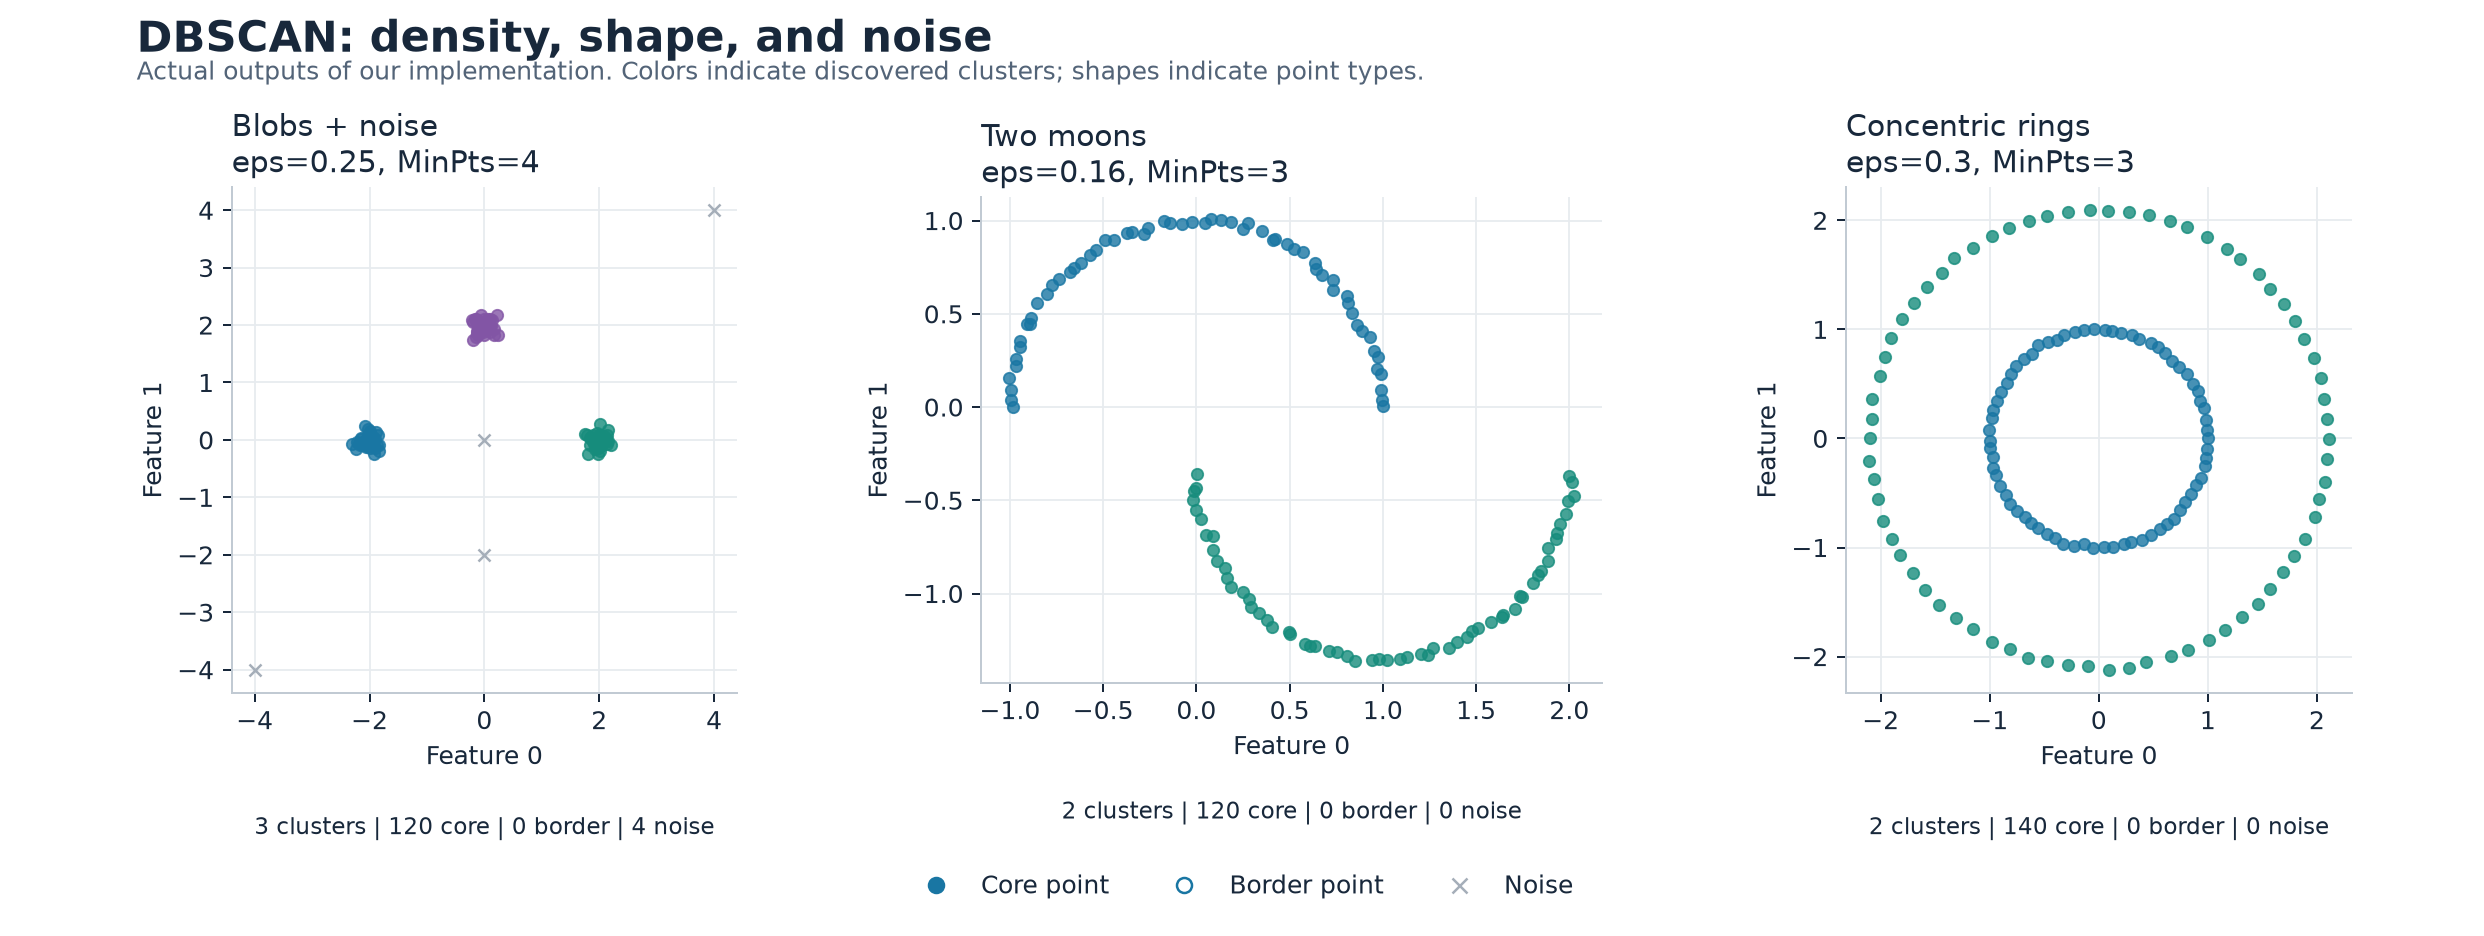
\includegraphics[width=\linewidth,keepaspectratio]{images/01_dbscan.png}
\end{center}
\vspace{-1em}

These representative settings come from the existing mock parameter
grid, with seed 7. The implementation finds three compact clusters and
four noise points, two curved moon-shaped clusters, and two concentric
rings. Cluster counts are discovered from density; they are not supplied
as inputs.

Filled circles denote core points, hollow circles denote border points,
and crosses denote noise. These particular settings produce no border
points; border classification, shared borders, and noise-to-border
reassignment are covered by the DBSCAN tests. Results depend on epsilon
and MinPts.

\clearpage

\subsection{Figure 1A: A Local Explanation of Core, Border, and Noise}
\figlabel{1A}{fig:local}

\begin{center}
    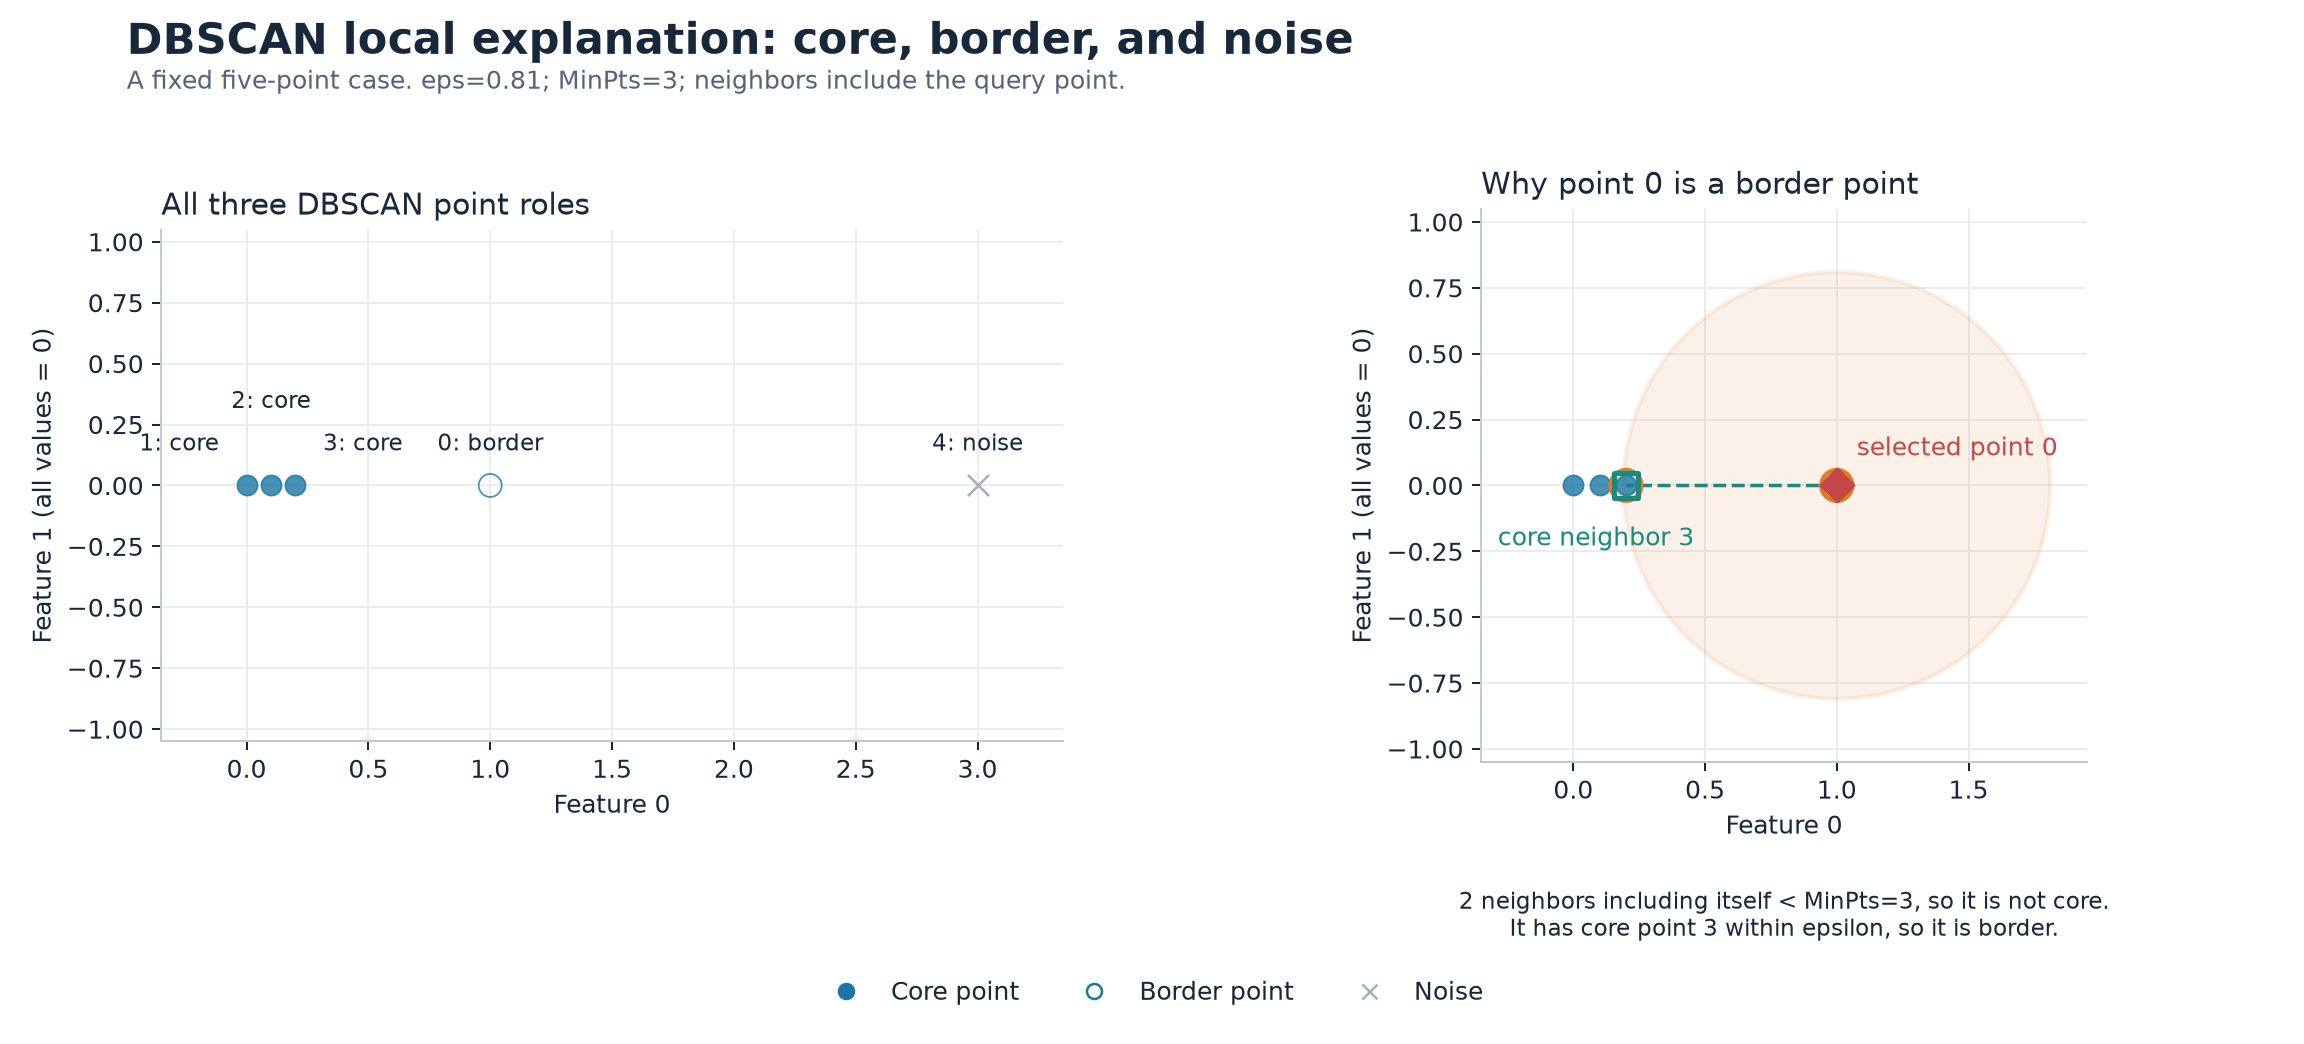
\includegraphics[width=\linewidth,keepaspectratio]{images/01a_dbscan_explanation.png}
\end{center}
\vspace{-2em}

This fixed five-point case contains three core points, one border point,
and one noise point. With epsilon=0.81 and MinPts=3, selected point 0 has
only two neighbors when the point itself is included, so it is not core.
It is nevertheless within the epsilon-neighborhood of core point 3 and is
therefore a border point. The distant point 4 has no neighboring core
point and remains noise.

The example is intentionally small enough to check by hand. The plotting
script asserts the point roles, neighbor counts, selected neighborhood,
and neighboring core point before producing the figure. It complements
the larger synthetic datasets used for parameter experiments.

\clearpage

\subsection{Figure 1B: Sweeping Epsilon and MinPts}
\figlabel{1B}{fig:sweep}

\begin{center}
    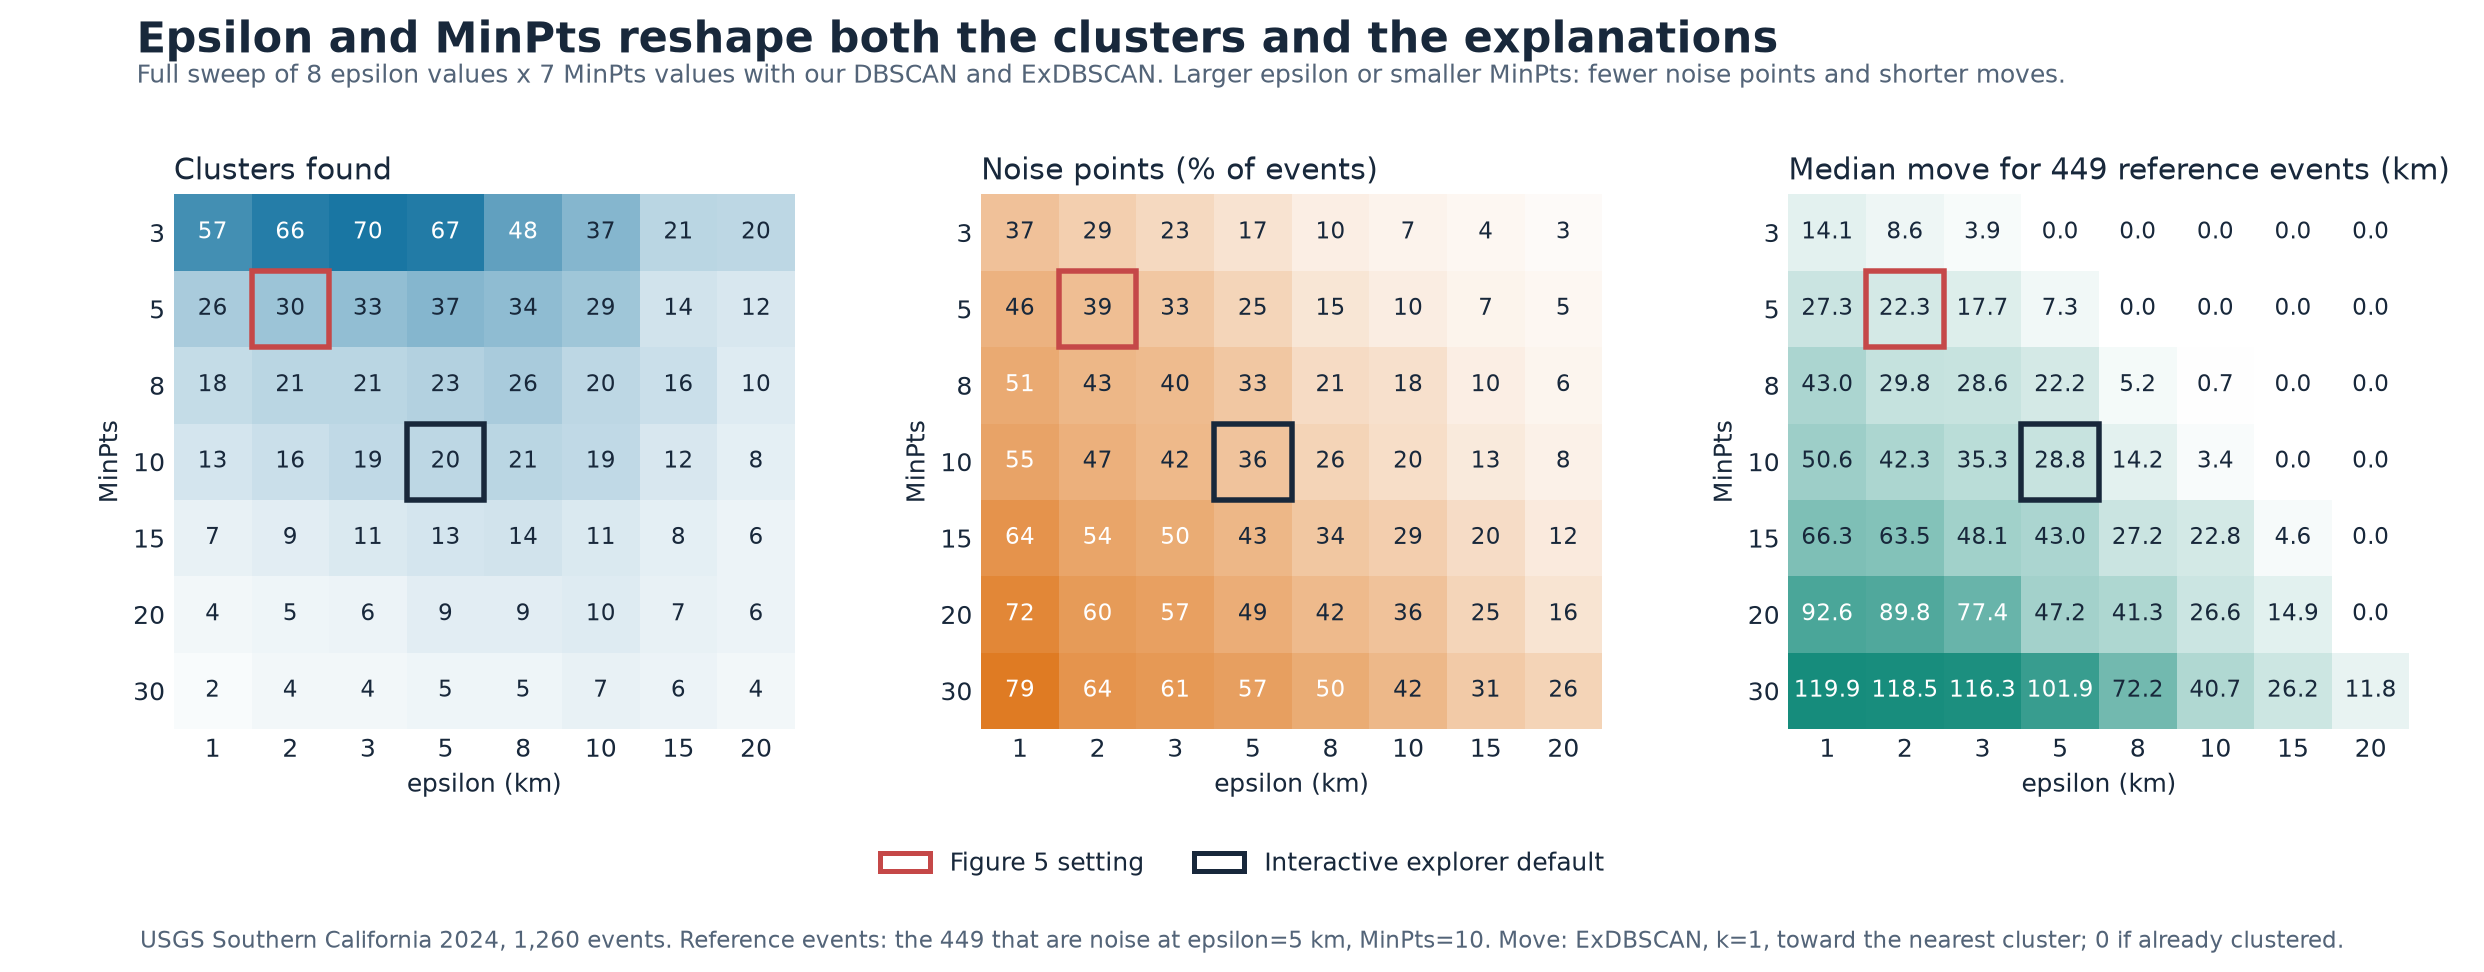
\includegraphics[width=\linewidth,height=100mm,keepaspectratio]{images/01b_parameter_sweep.png}
\end{center}

All 56 settings (8 epsilon values and 7 MinPts values) were run with our
DBSCAN on the 1,260 USGS events. The cluster count is not monotone in
epsilon: with MinPts=5 it rises from 26 to 37 and then falls to 12 as
clusters merge. Noise ranges from 2.7\% to 79.4\%. The red box is the
setting of Figure 5 (30 clusters); the black box is the interactive
explorer default (20 clusters, 35.6\% noise).

The right panel fixes the 449 events that are noise at the explorer default
and asks how far each must move, with ExDBSCAN and k=1, to join the nearest
cluster under every other setting (0 if it is no longer noise). The median is
28.8~km at the default and drops to 0 once epsilon is large or MinPts small.
For k=1 this equals the distance to the nearest core point minus epsilon,
which the script asserts. It is one snapshot, so it shows the trend, not a
general rule.

\clearpage

\subsection{Figure 1C: Where DBSCAN Is Fragile}
\figlabel{1C}{fig:limits}

\begin{center}
    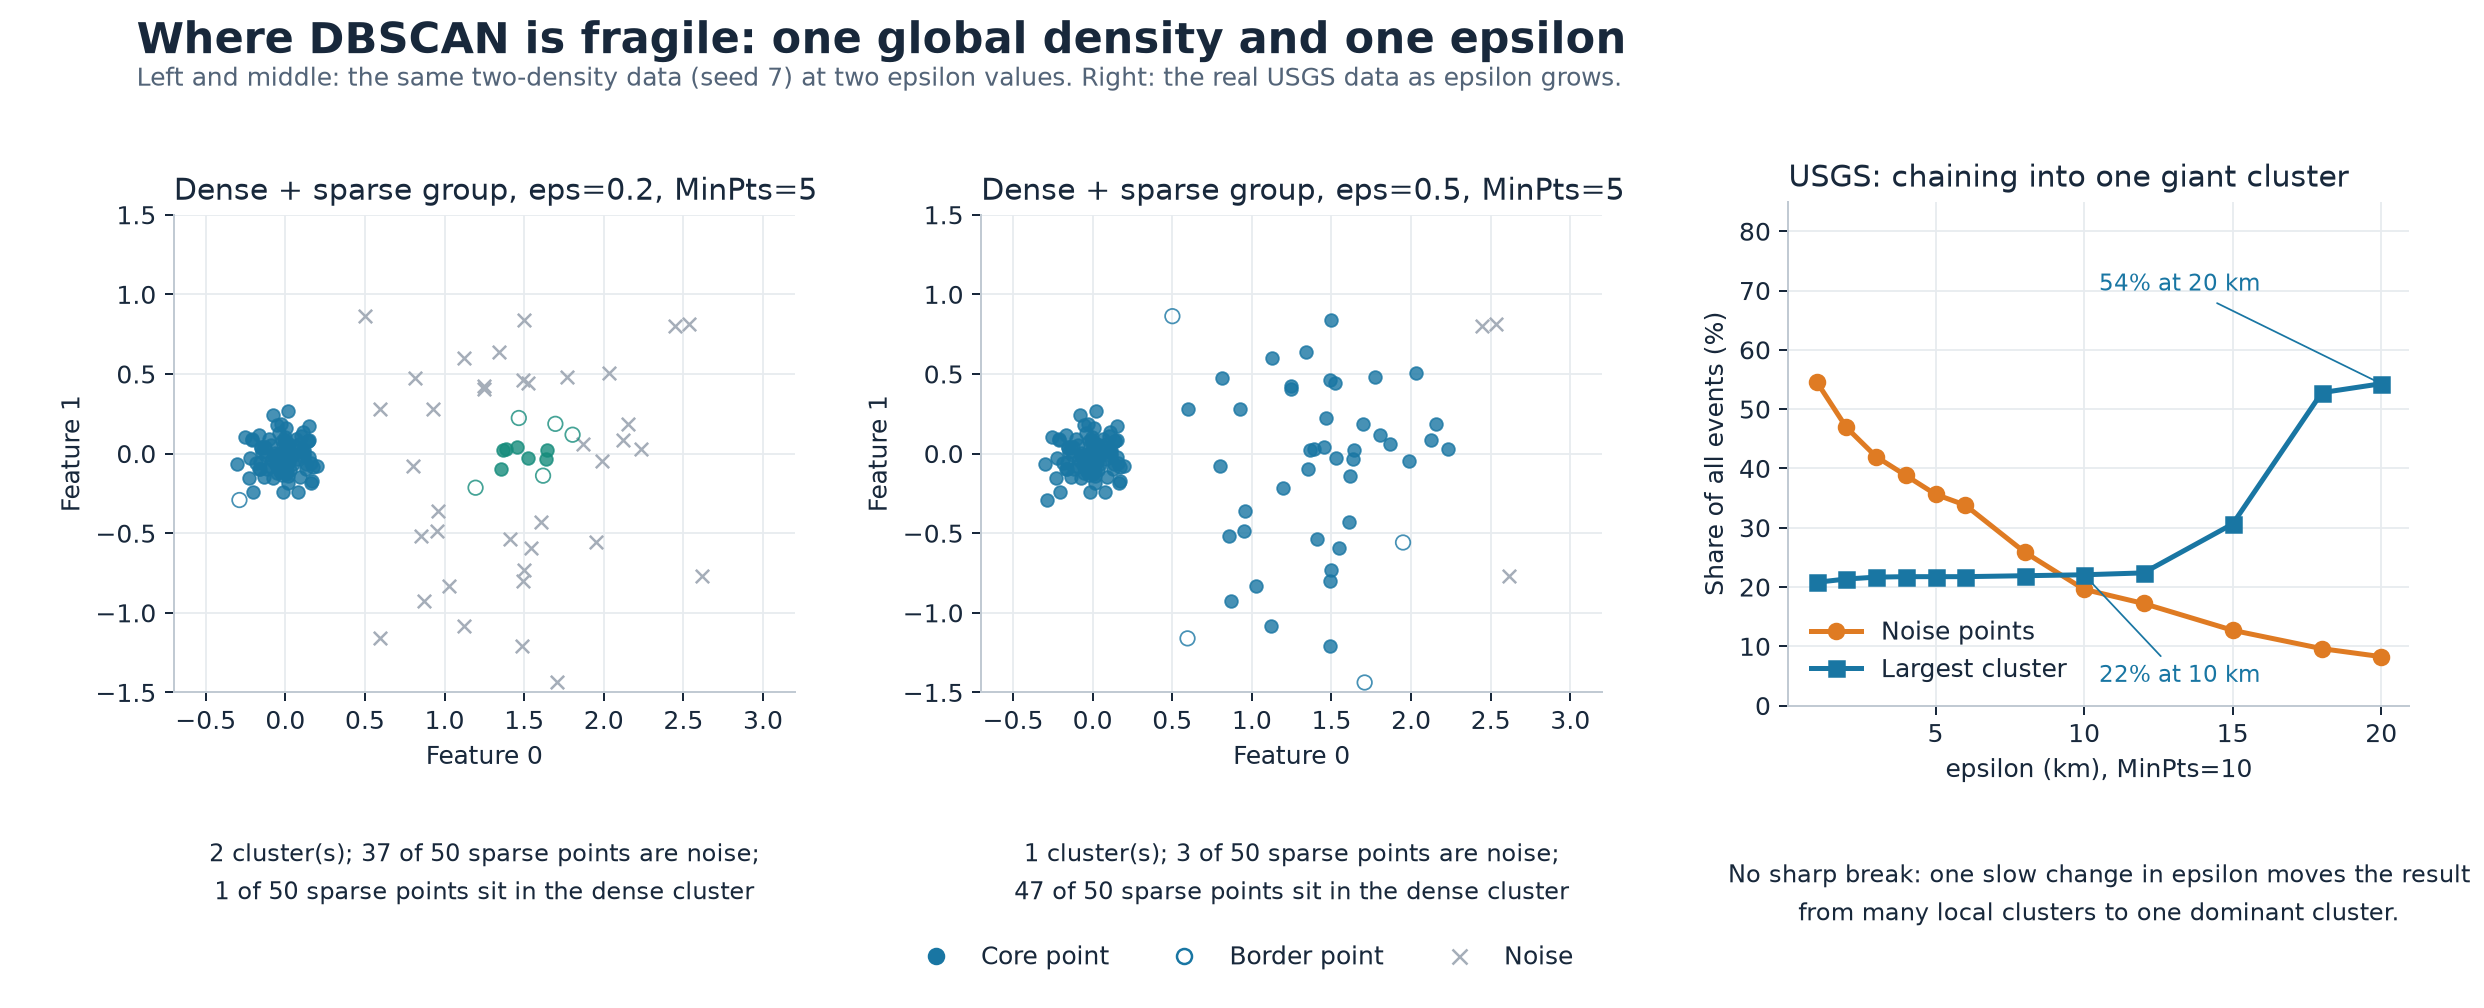
\includegraphics[width=\linewidth,height=96mm,keepaspectratio]{images/01c_limitations.png}
\end{center}

\textbf{Varying density.} The synthetic data (seed 7) has a dense group and a
sparse group. With epsilon=0.2, 37 of the 50 sparse points are noise. With
epsilon=0.5, the two groups merge into one cluster. Epsilon=0.4 separates
them (2 clusters, 7 sparse noise points), so a window exists, but it is narrow
and one global epsilon has to be chosen for both densities.

\textbf{Chaining.} On the USGS data (MinPts=10) the largest cluster holds 22\%
of the events at 10~km, 31\% at 15~km, and 54\% at 20~km, while noise falls
from 20\% to 8\%. Because ExDBSCAN explains a fixed clustering, these effects
carry over to its counterfactuals.

\clearpage

\subsection{Figure 2: Core Graph, Reference Selection, and Counterfactuals}
\figlabel{2}{fig:exdbscan}

\begin{center}
    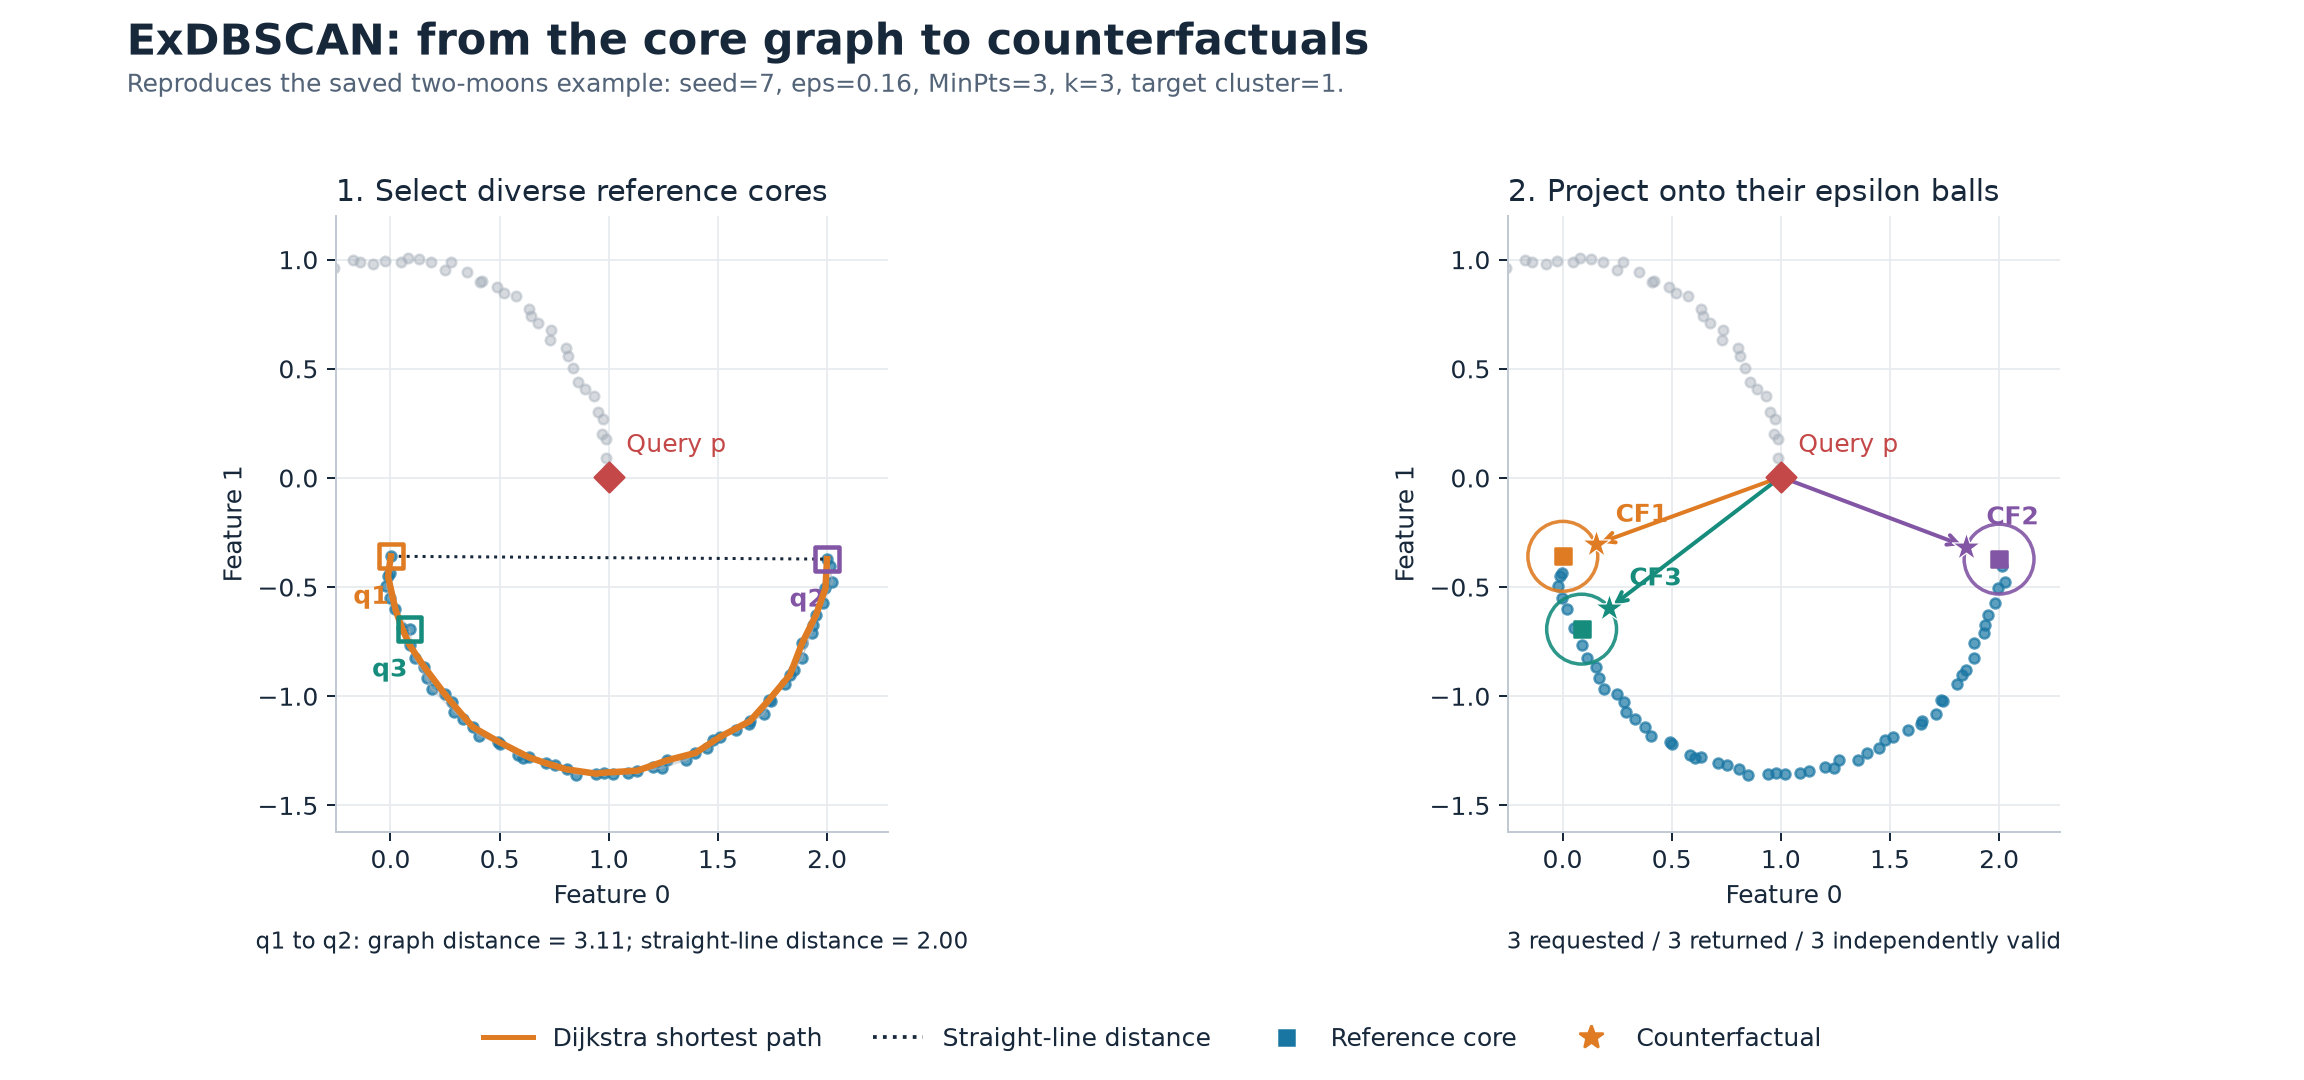
\includegraphics[width=\linewidth,height=100mm,keepaspectratio]{images/02_exdbscan.png}
\end{center}
\vspace{-2em}

The red diamond is the query p. The left panel shows three reference
core points selected by the implemented greedy objective. The orange
path between q1 and q2 is recovered from our Dijkstra distance labels:
its length is approximately 3.11, compared with a straight-line distance
of approximately 2.00. This shows why graph distance captures the target
cluster\textquotesingle s curved structure.

The right panel projects the query toward the epsilon ball of each
selected reference. Stars denote three distinct counterfactuals, all
independently verified to reach the requested target cluster. Arrows
represent feature changes, not constrained travel paths. This example is
regenerated from the parameters in \texttt{results/mock\_examples.json}
and checked against its saved coordinates and reference indices.

This demonstrates multiple explanations and graph-based diversity
selection; it does not prove global optimality for k \textgreater{} 1 or
superiority over every baseline.

\clearpage

\subsection{Figure 3: Immutable Features and Infeasibility}
\figlabel{3}{fig:constraints}

\begin{center}
    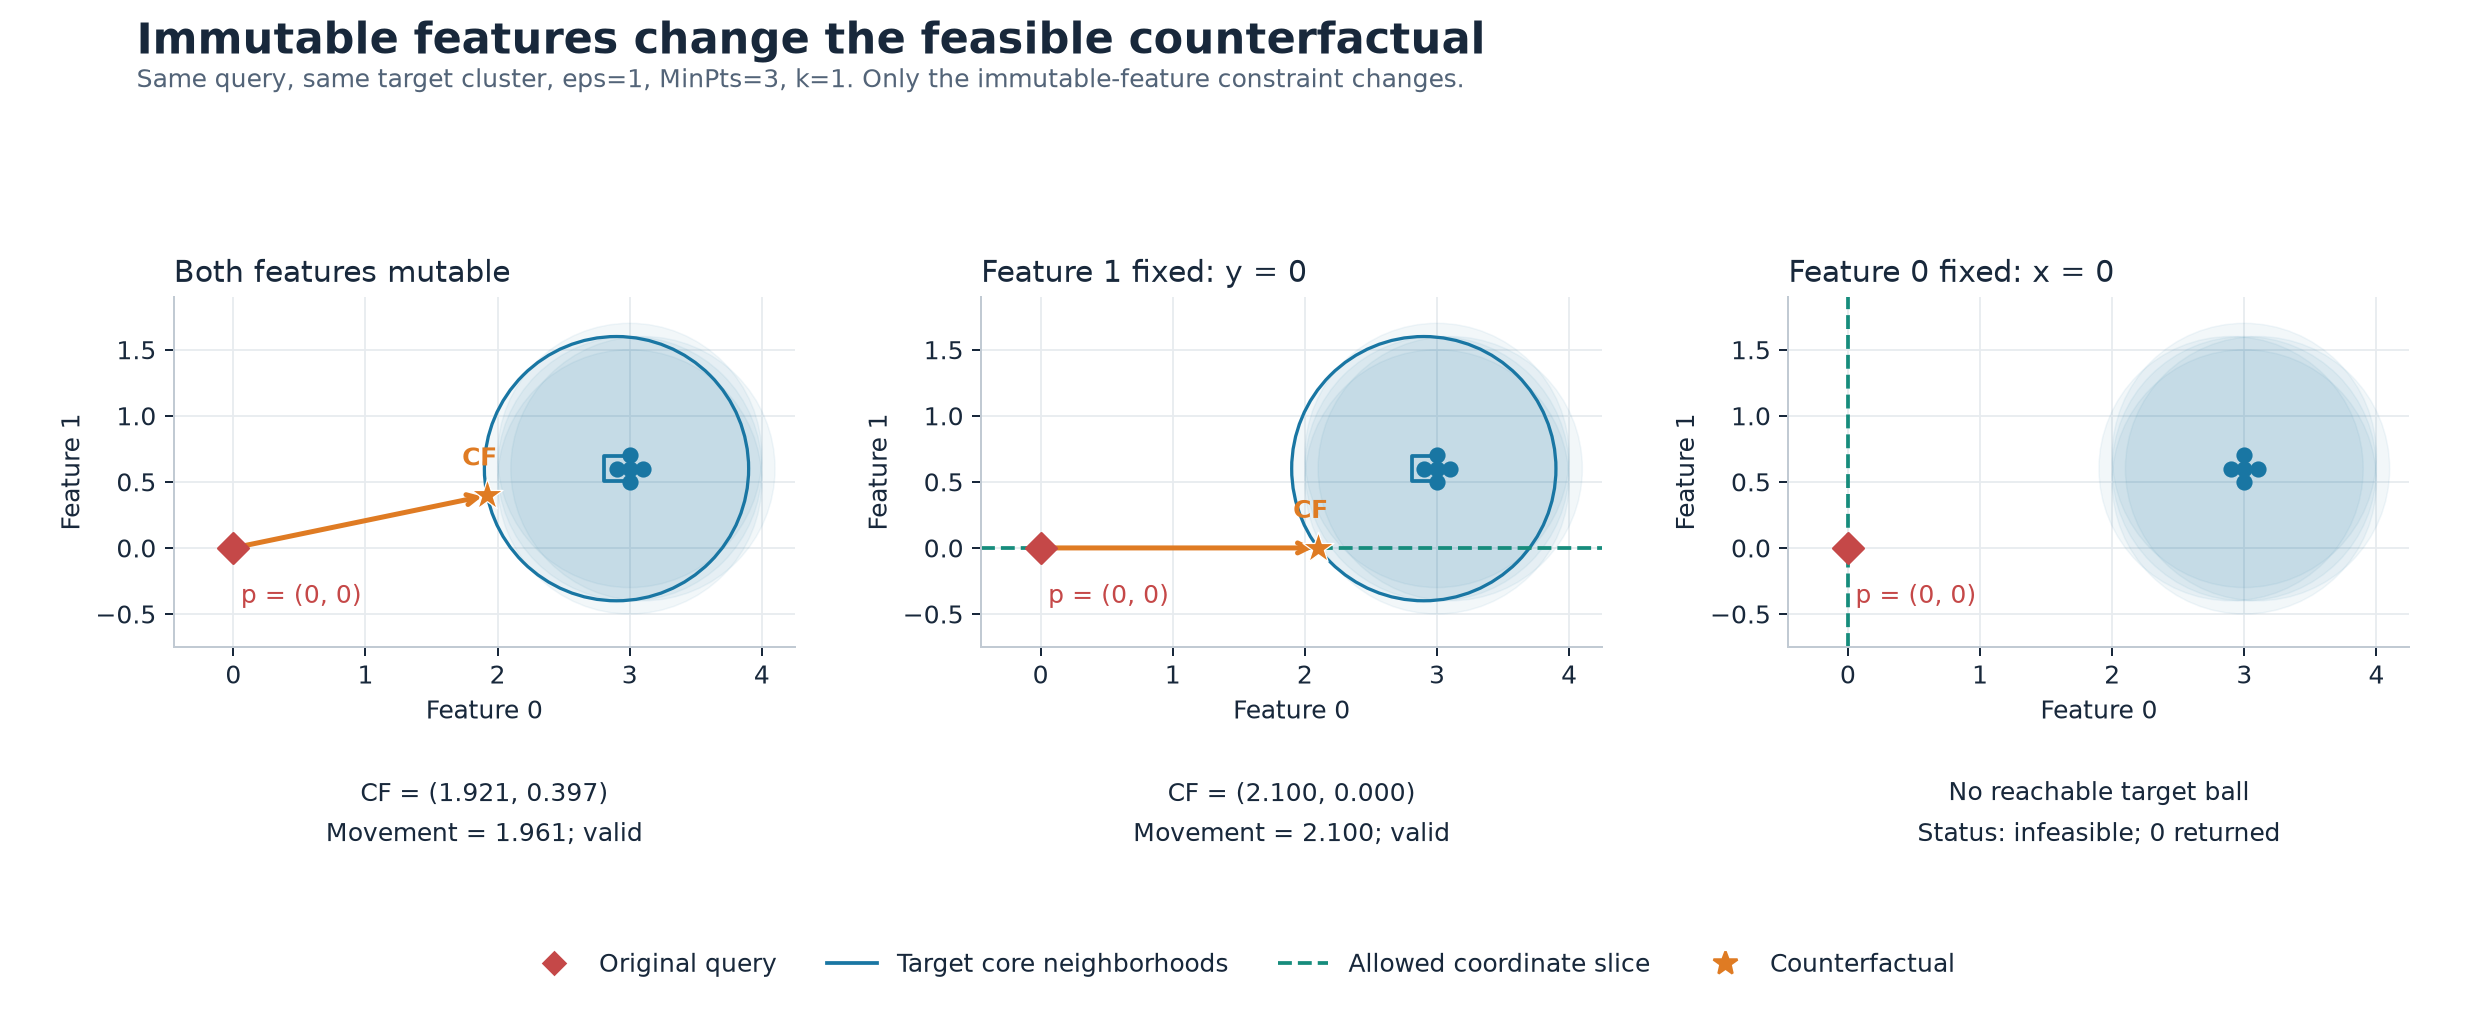
\includegraphics[width=\linewidth,height=100mm,keepaspectratio]{images/03_constraints.png}
\end{center}
\vspace{-2em}

The query is (0, 0), the target points lie near (3, 0.6), epsilon=1,
MinPts=3, and k=1 in every panel.

\begin{longtable}[]{@{}p{0.19\linewidth}p{0.25\linewidth}p{0.18\linewidth}p{0.32\linewidth}@{}}
    \toprule\noalign{}
    Constraint           & Counterfactual               & Euclidean movement & Result                  \\
    \midrule\noalign{}
    \endhead
    \bottomrule\noalign{}
    \endlastfoot
    None                 & Approximately (1.921, 0.397) & 1.961              & Valid                   \\
    Feature 1 fixed at 0 & (2.100, 0.000)               & 2.100              & Valid; fixed coordinate
    preserved exactly                                                                                  \\
    Feature 0 fixed at 0 & None                         & Not applicable     & Infeasible              \\
\end{longtable}

Freezing y restricts movement to the horizontal dashed line, increasing
the required change in this example. Freezing x restricts movement to
the vertical line, which never intersects a target core ball. The
correct outcome is an infeasible status with no counterfactual. This is
a separate small geometry demonstration, not an additional row in the
benchmark totals.

\clearpage

\subsection{Figure 4: Validity, Coverage, and Complete Requests}
\figlabel{4}{fig:validation}

\begin{center}
    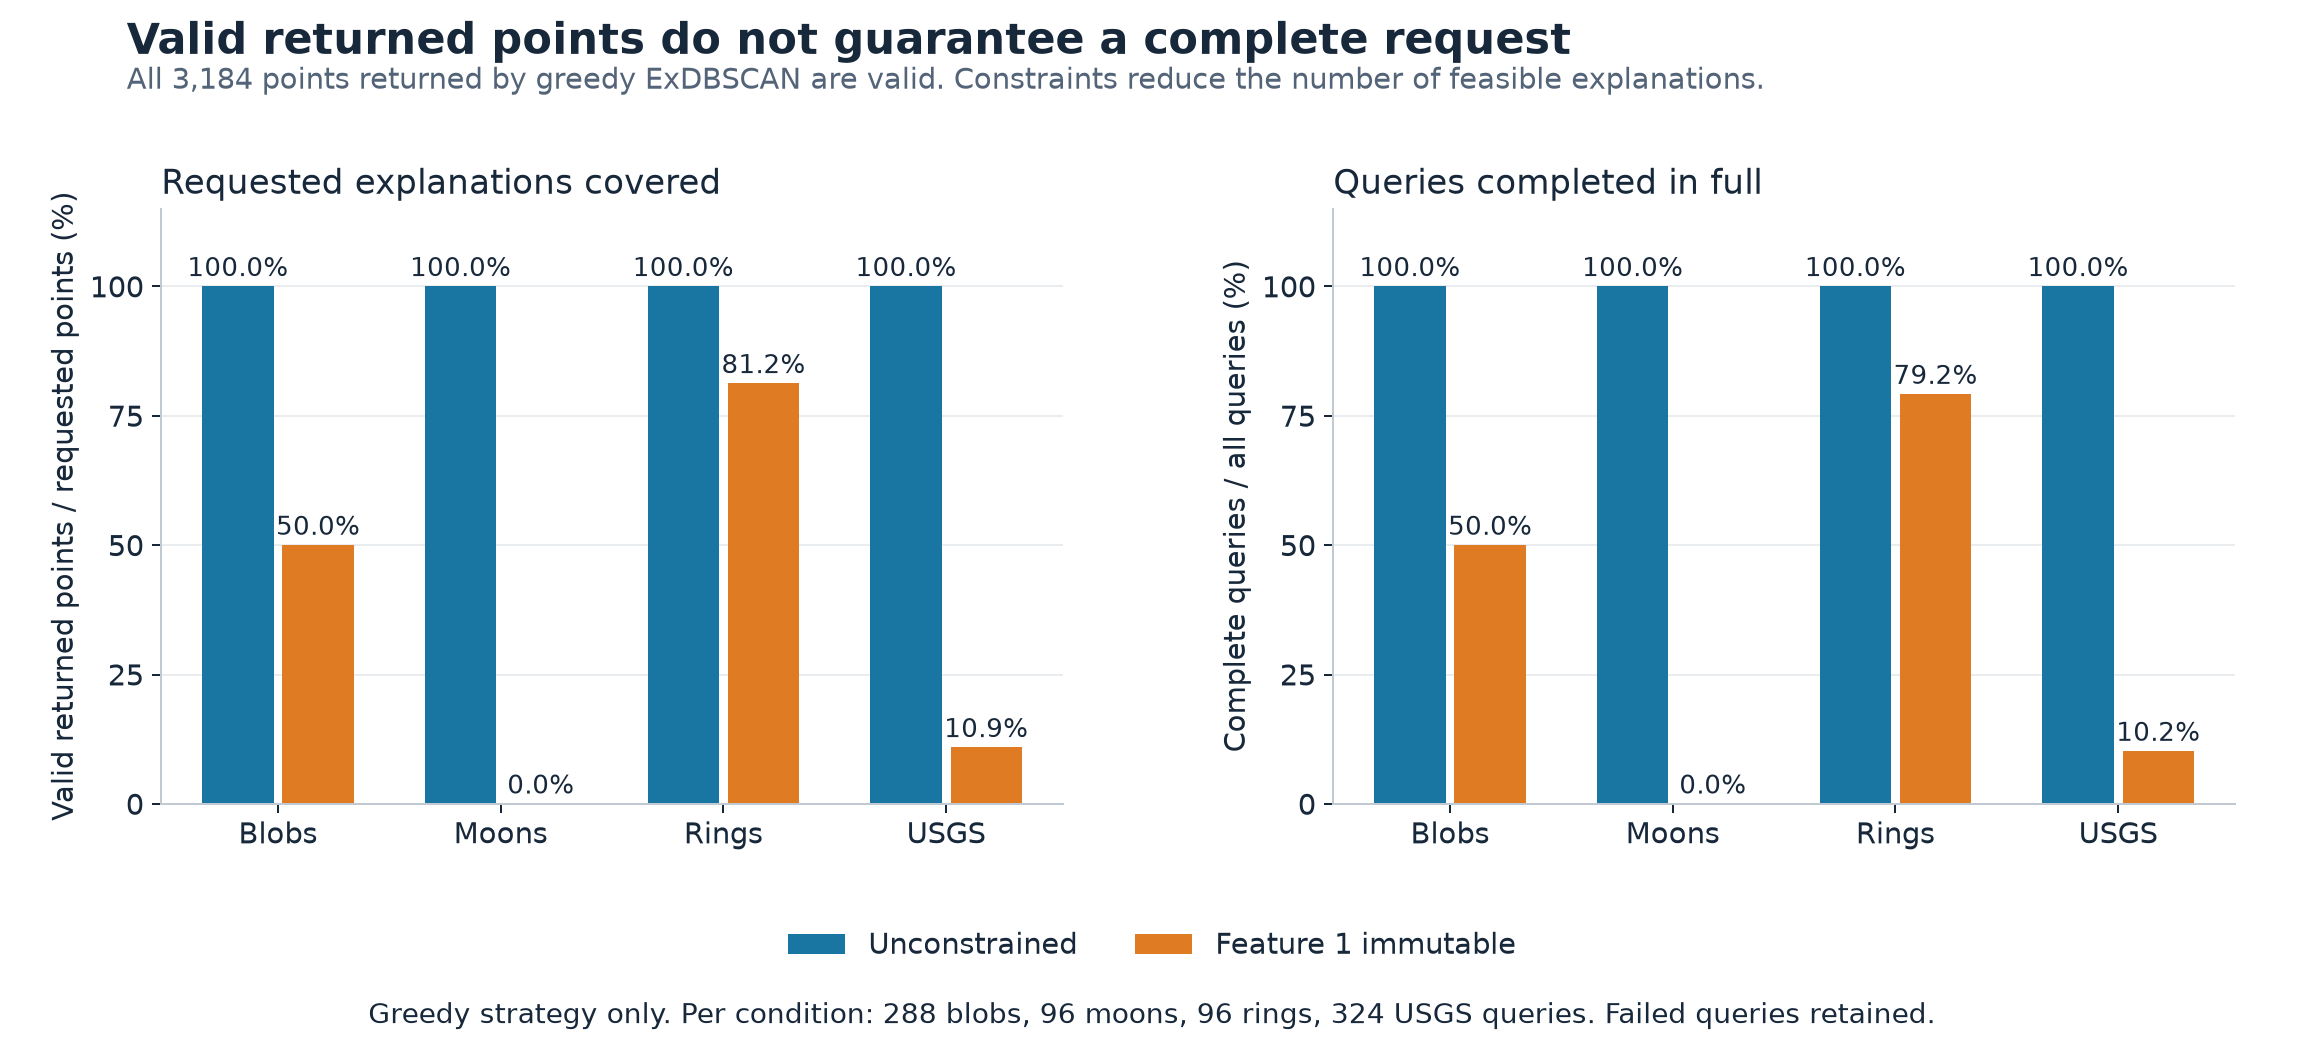
\includegraphics[width=\linewidth,height=80mm,keepaspectratio]{images/04_validation.png}
\end{center}
\vspace{-2em}

This figure isolates the \textbf{greedy ExDBSCAN strategy}: 1,608
queries and 3,184 returned points. All returned points are valid. The
larger totals at the top of this document also include the nearest and
random baseline strategies.

\begin{itemize}
    \tightlist
    \item
          \textbf{Requested coverage} is the number of valid returned points
          divided by the total number requested. A partial result contributes
          only its valid points.
    \item
          \textbf{Complete-query rate} is the proportion of queries that return
          all k requested points and pass every validity check.
\end{itemize}

For the tested unconstrained queries, both measures are 100\%. With
feature 1 fixed, requested coverage is 50.00\% for blobs, 0.00\% for
moons, 81.25\% for rings, and 10.91\% for USGS. Complete-query rates are
50.00\%, 0.00\%, 79.17\%, and 10.19\%, respectively. Rings and USGS
include partial results, which explains the difference between their two
measures.

The fixed-y moon queries in this sample cannot reach their requested
target clusters. Their zero coverage describes these sampled queries and
settings, not a claim that all constrained moon datasets are infeasible.
They return no points, so there is no nonempty returned set from which
to estimate validity. Failed and partial queries remain in the
statistics.

\clearpage

\subsection{Figure 5: Real Spatial Data}
\figlabel{5}{fig:real}

\begin{center}
    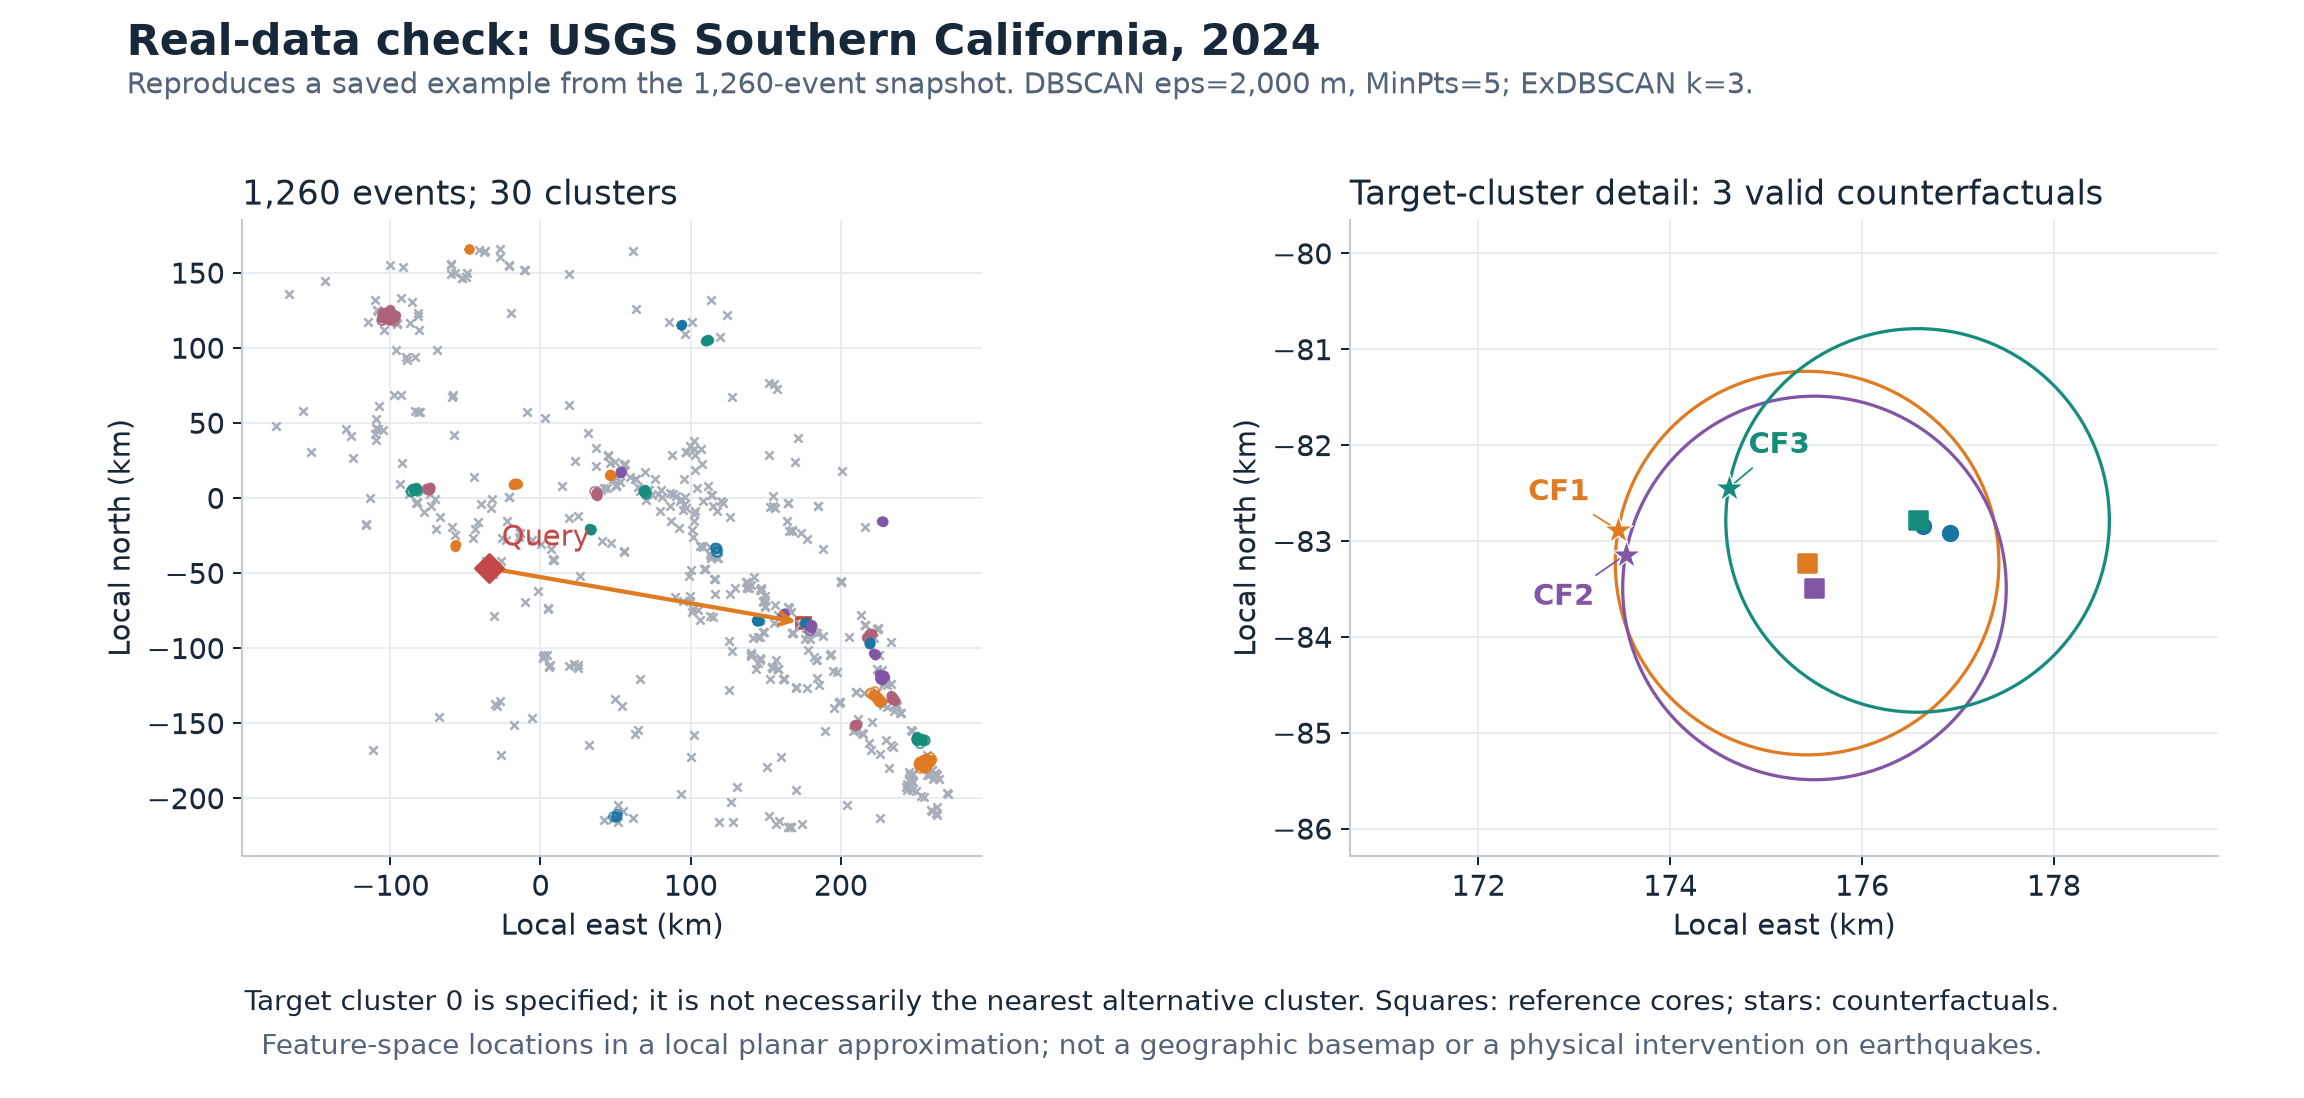
\includegraphics[width=\linewidth,height=110mm,keepaspectratio]{images/05_real_data.png}
\end{center}
\vspace{-1em}

The left panel uses all 1,260 locations in the recorded USGS Southern
California 2024 snapshot. At epsilon=2,000 meters and MinPts=5, our
DBSCAN finds 30 clusters. The right panel magnifies the specified target
cluster and shows three validated counterfactuals. This reproduces a
saved real-data example, including its reference indices and output
coordinates.

The specified target is cluster 0, which need not be the nearest
alternative cluster. The large movement in the overview therefore must
not be interpreted as the minimum change needed to reach any cluster.
Axes show local projected coordinates in kilometers; clustering still
uses meters. This is a feature-space plot, not a geographic basemap or
an actionable intervention on earthquakes.

\clearpage

\subsection{Reproduce and Reuse the Figures}
\label{reproduce-and-reuse-the-figures}

From the project root, after validation and both experiment stages have
passed:

\begin{codebox}
    \begin{Verbatim}[fontsize=\small,commandchars=\\\{\}]
        \codecomment{# Optional plotting dependency; not required by either algorithm}
        python3 -m pip install matplotlib
        python3 examples/plot_results.py

        \codecomment{# Figure 1A can be regenerated independently}
        python3 examples/plot_dbscan_explanation.py
    \end{Verbatim}
\end{codebox}

The original script writes five PNG images and five editable vector SVG files to
\texttt{results/figures/}. It also writes
\texttt{results/visual\_examples.json}, which records the demonstration
outputs, independent metrics, shortest-path evidence, plotting runtime,
source fingerprint, script hash, and figure hashes. Saved aggregate
counts are cross-checked against the query CSVs, and the real-data
snapshot hash is checked before plotting.

The separate \texttt{plot\_dbscan\_explanation.py} script produces Figure 1A
without rerunning or changing the saved experiments or their five figures.
It records the five-point input, DBSCAN output, neighborhood checks,
rendering runtime, and figure hashes in
\texttt{results/dbscan\_local\_example.json}.

The plot-generation runtime can differ from the algorithm-test runtime;
both are recorded separately. Existing tests, experiment results, and
algorithm source code are not modified by plotting.

For parameter grids and limitations, see \href{../experiment_plan.md}{the experiment plan}, \href{../method_spec.md}{the method specification}, and \href{../validation_report.md}{the validation report}.

\end{document}
